\maketitle
\section{Resampling Study}

To test the ecological validity of findings in experiment 1 and 2 we have also designed a
resampling study based on European Values Survey data.
By using data gathered for an actual survey, we can mostly observe whether the relative 
performances of the imputation methods change when they are deployed for real data research.
Variables in the EVS data are not generated artificially from continuously normal distributions 
but are discrete numerical items that are treated as such by researchers.

The resampling study follows a similar strategy to that used in the simulations. 
To assess the statistical validity of the different imputation methods we have repeated the 
following steps 1000 times ($R = 1000$):

\begin{itemize}
	\item Data generation - A bootstrap sample $\bm{X}^{*}$ was generated by sampling with replacement $n$ 
		observations from a pre-processed EVS data-matrix. 
		Part of the pre-processing step was some form of imputation used to obtain a pseudo-fully observed 
		input data matrix.
	\item Missing data imposition - Missing values were imposed on a given number of target variables
		in $\bm{X}^{*}$, according to some response model.
	\item Imputations - Each method described in section 2 to deal with missing values was used to impute
		NAs.
	\item Analysis - Two analysis models were fitted to the differently treated data.
		Parameters estimates pooled across the differently imputed datasets for the MI methods and
		stored along with the estimates obtained with single imputation methods and complete case 
		analysis.
\end{itemize}

	The average estimate, over the $R$ repetitions, obtained with the Gold Standard approach are considered 
	as "true" reference values of the parameters in the analysis models.
	The $R$ estimates obtained with all other methods are used to obtain performance measures for each imputation 
	method using the same criteria described for study 1 and 2 (see \ref{criteria}).

	The code to Run the simulation was written in the R statistical programming language (version 4.0.3). 
	The resampling study was run using a 2.6 GHz Intel Xeon(R) Gold 6126 processor, 523780 MB of Memory. The
	operating system was Windows Server 2012 R2.

	Computations were run in parallel across the available cores (between 30). Parallel computing 
	was implemented using the R package 'parallel' and to ensure replicability of the findings seeds were
	set using the method by \cite{lecuyer:2002} implemented in the R package 'rlecuyer'

\subsection{Methods}

\paragraph{Data preparation}
	EVS is a standardizes cross-sectional survey with a representative sample of more than 60,000 
	people, across more than 30 countries, interviewed via Web, post or face-to-face.
	For this study we have used the third pre-release of the 2017 wave of EVS data \citep{EVS:2017}.
	The original dataset contained 55,000 observations in 34 countries.

	We selected only the four European Founding Countries included in the data (France, Germany,
	Italy, and the Netherlands) and excluded all columns of the data that were either duplicated
	information (recoded versions of other variables), or linked to meta data (e.g. time of interview,
	mode of data collection). 
	All missing values were filled in with a run of a single imputation predictive mean matching (PMM) 
	which allowed us to obtain a pseudo fully-observed dataset. PMM was chosen for the task as it 
	is an effective, flexible imputation method that maintains the distributional characteristics of 
	the original data. 
	The full cleaning process is more systematically described in the appendix.

	At the end of this data cleaning process, we ended up with a fully-observed dataset
	of 8045 observations ($n$), across 4 countries, and 243 variables ($p$).

\paragraph{Analysis model(s)}

	To define plausible analysis models we have searched the EVS database for articles using
	such data looking for suitable analysis models on which to test the effectiveness of 
	the different imputation algorithm.
	We have defined two linear regression models of the form:
	\begin{center}
		\begin{equation} \label{eqn:lm}
			\bm{y} \sim \beta_0 + \bm{\beta_1} \bm{x}_1 + \bm{\beta}_{-1} \bm{X}_{-1}
		\end{equation}
	\end{center}

	In model 1, inspired by \cite{koneke:2014}, the dependent variable is a 10-point EVS item measuring euthanasia 
	acceptance ('Can this always be justified, never be justified, or something in between?'); the predictor 
	of interest a 4-point item measuring the self-reported importance of religion in one's life.
	A variety of covariates, such as measures of trust, education, and socio-economic status, were included in 
	$\bm{X}_{-1}$ as control variables.

	This model represents a plausible analysis a researcher would perform to test a theory regarding the 
	effect of religiosity on end-of-life treatments.

	In model 2, inspired by \cite{immerzeel:2015}, the dependent variable is an harmonized variable
	constructed by EVS to describe the respondents' tendency to vote on a 10-point left-to-right continuum; 
	the predictor of interest is a composite mean scale measuring respondents attitudes toward immigrants 
	and immigration ('nativist attitudes scale').
	Respondents expressed how much they agreed on a scale from 1 to 10, with the following statements: 
	'immigrants take jobs away from natives', 'immigrants increase crime problems', and 
	'immigrants are a strain on welfare system'.
	The control variables used included the usual socio-economic background information, the same measure of
	religiosity used in model 1, and some measures of political interest.

	A research might fit this model to their data and look at the regression coefficient of the nativist attitudes
	scale to test some theory regarding its effect on voting for right wing parties.

\paragraph{Missing data imposition}

	Missing data were imposed on 6 variables according to the same strategy as in \ref{subsub_missing}.
	The target variables we identified were the two dependent variables in models 1 and 2, religiosity (predictor
	in both models) and the three items making up the nativist attitudes scale (predictor in the second model).

	The response model form is the same as in \label{eqn:rm} and 3 variables were included in $\tilde{X}$: 
	age, education, and an item measuring trust in new people. 
	These are plausible variable that influence response tendencies in participants: 
	older people usually have higher item non-response rates than younger;
	so do lower educated compared to higher educated people; 
	people that have less trust in new people are assumed to withhold more information from the interviewer.

\paragraph{Conditions}
	There were only two conditions for the resampling study: low and high dimensional imputation.
	As the number of predictors in the data is fixed ($p = 250$), the dimensionality of the data is
	changed by defining different sizes for the sample taken from the pseudo-fully observed data.
	We chose only two values for $n$, namely $1000$ and $300$, corresponding to the low and high 
	dimensional condition.

\subsection{Results}
\subsubsection{Bias}

	\paragraph{PRB}
	Figure \ref{fig:exp4bias} reports the PRB for the regression coefficients of interest in model 1 and 2.
	Most of the MI methods result in negligible biases ($PRB < 10\%$) for both parameters in all conditions.
	The only two exceptions are bridge and MI-RF: the former is very competitive in condition (a), the low
	dimensional one, but leads to extreme bias in the high dimensional condition (b); the latter provides, 
	in all conditions, the highest PRB among the MI methods, it is consistently outperformed even by
	Complete Case analysis, and results in a 10\% PRB for the regression coefficient of nativist attitudes 
	in model 2.

	DURR and IURR are giving inconsequential biases for both parameters in all conditions, with PRBs that are
	often at least half in size as the ones obtain with the other methods.

	\paragraph{Euclidean Distance}
	Figure \ref{fig:exp4biased} reports the Euclidean Distance between the vector of estimated regression 
	coefficients for model 1 and 2.
	IURR and DURR yielded the vectors of parameters estimates that are closer to the vector of true values.
	The advantage in using these methods over others is stark for model 2 while it is less marked in model 1.
	While in the low dimensional condition, IURR does not seem to provide a lower bias than the other 
	methods, its relative performance improves as the dimensionality of the data increases.

	MI-PCA seems to struggle with bias for model 1, ranking last among the multiple imputation models.
	Nevertheless, it does provide a stark advantage compared to mean imputation and Complete Case analysis.

	Single imputation missForest is also able to provide a competitive vector of estimates, at least in model 2.

\begin{figure}
	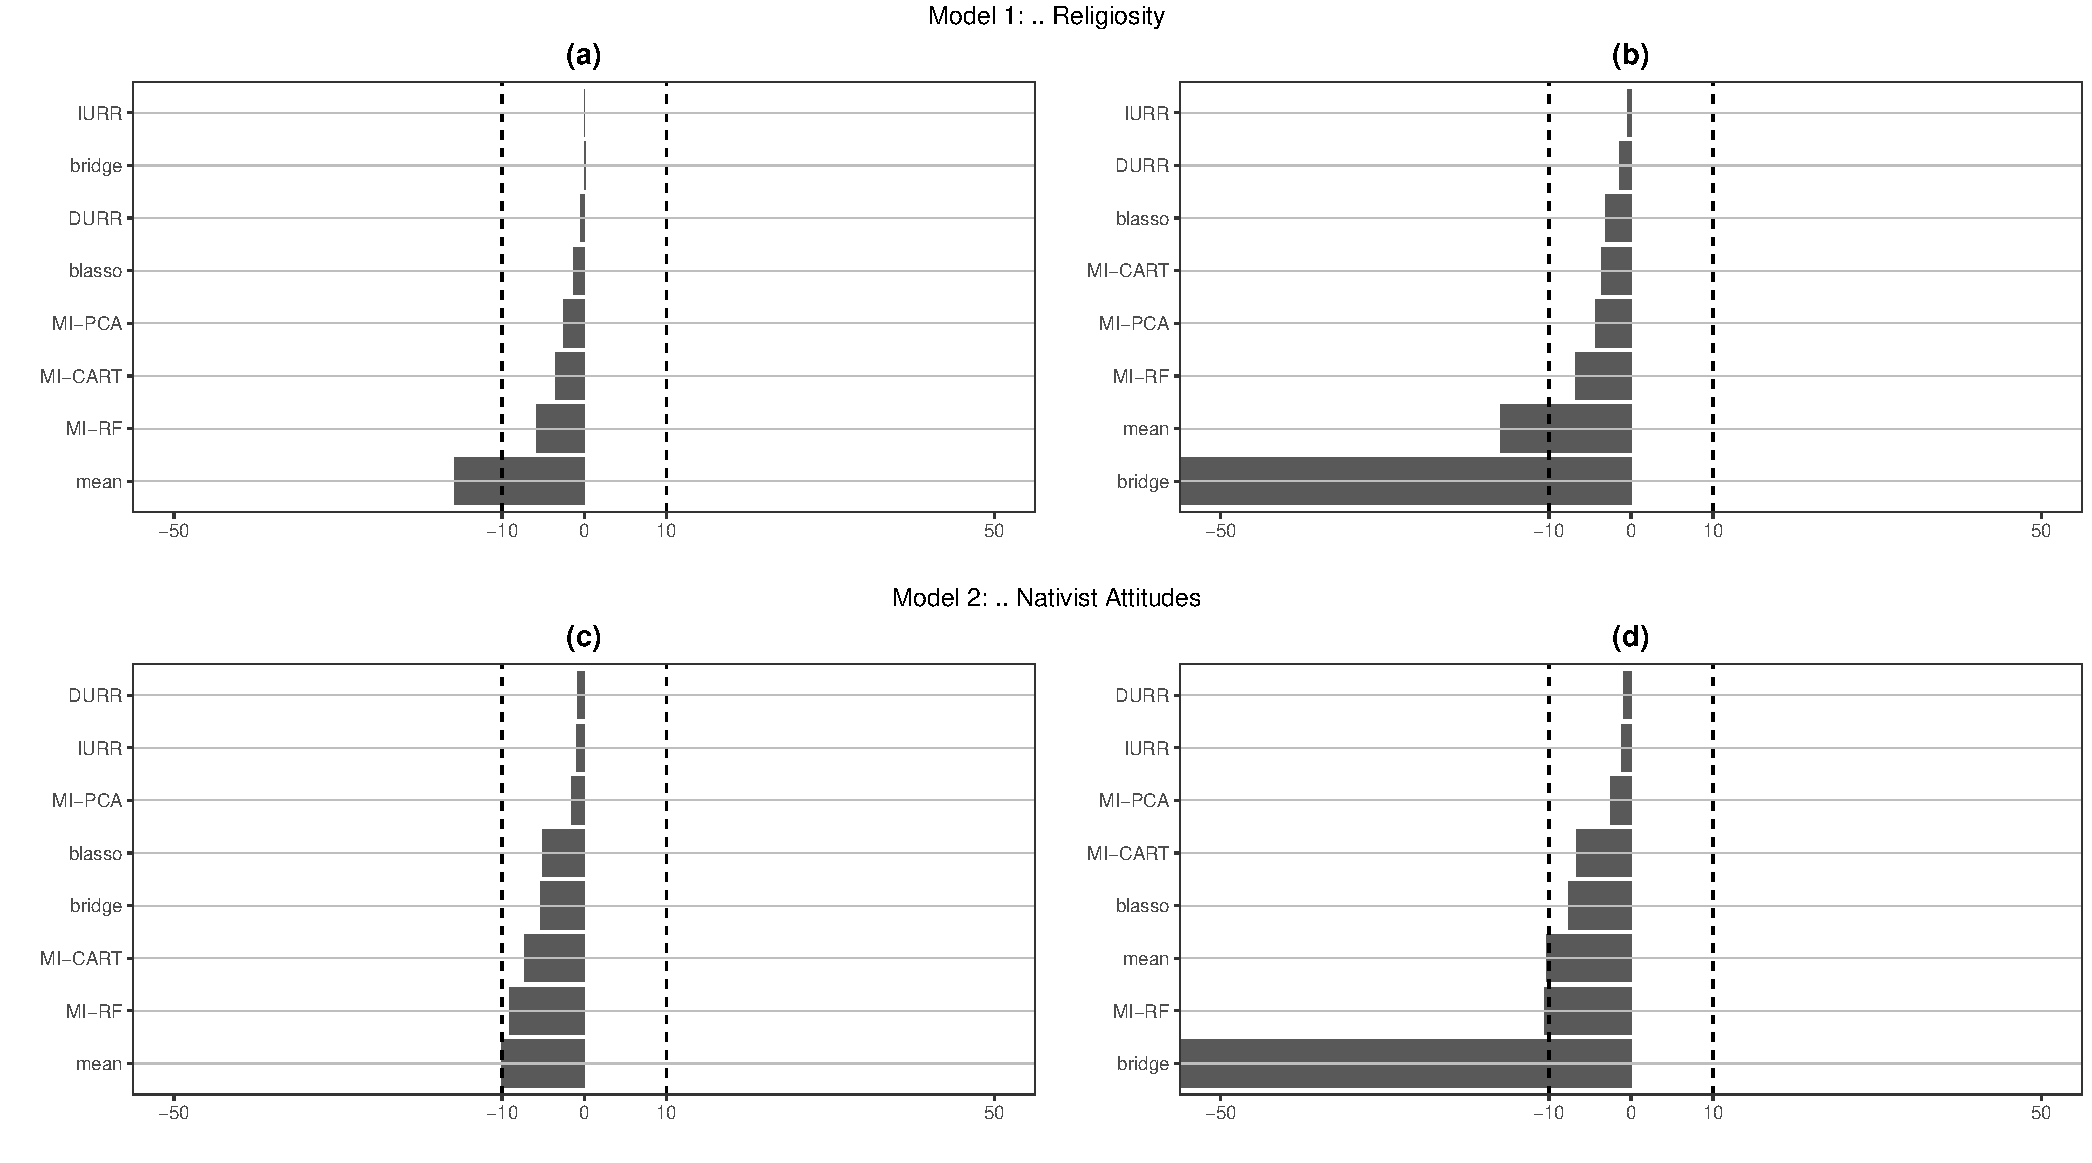
\includegraphics[width=\textwidth]{\pathFIG/exp4_imp_bias.pdf}
	\caption{Bias for single parameter of interest in the two different models}
	\label{fig:exp4bias}
\end{figure}

\begin{figure}
	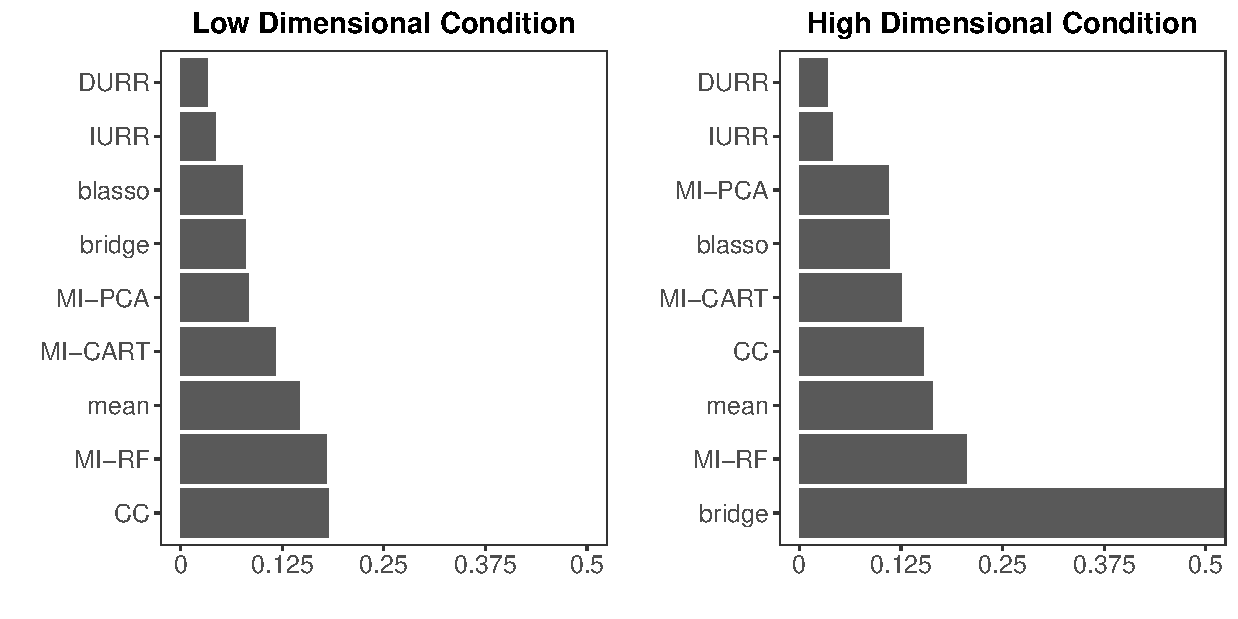
\includegraphics[width=\textwidth]{\pathFIG/exp4_ed_bias.pdf}
	\caption{Euclidean distance between the vector of estimated regression coefficients and
		the vector of their true value}
	\label{fig:exp4biased}
\end{figure}

\FloatBarrier

\subsubsection{Confidence Interval Coverage}

	\paragraph{Confidence Interval Coverage}
	Researchers interested in testing their theories with the inferential models described, will be interested
	in the confidence interval coverage of the estimates of interest.
	Figure \ref{fig:exp4ci} reports the CIR for the focal regression coefficient in the two models.

	Both IURR and DURR remain fairly competitive in terms of CIR, but the advantage they showed in terms of bias
	is not carried over to this criterion.
	Both MI-PCA and Blasso outperform IURR and DURR in almost all conditions, granting confidence intervals that 
	are noticeably closer to nominal coverage.
	
	\paragraph{Euclidean Distance}
	However, when looking at a more general pattern reported in \ref{fig:exp4cied}, IURR and DURR return to 
	the top of the leader-board, providing the closest vectors of Confidence Interval Coverages for model parameters 
	to nominal levels.

	\paragraph{Confidence Interval Width}
	Plot?

\begin{figure}
	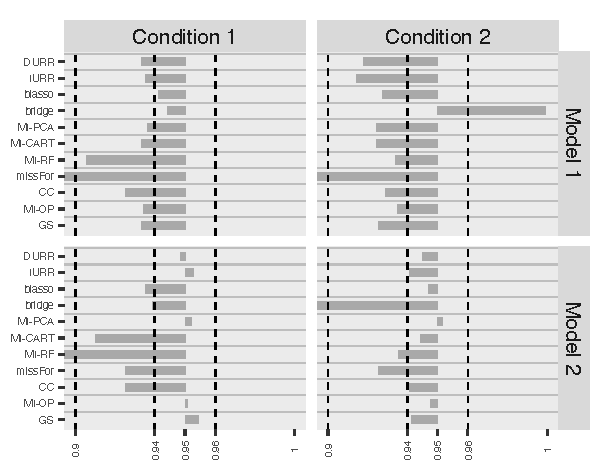
\includegraphics[width=\textwidth]{\pathFIG/exp4_imp_ci.pdf}
	\caption{Confidence Interval Coverage for single parameter of interest in the two 
		different models}
	\label{fig:exp4ci}
\end{figure}

\begin{figure}
	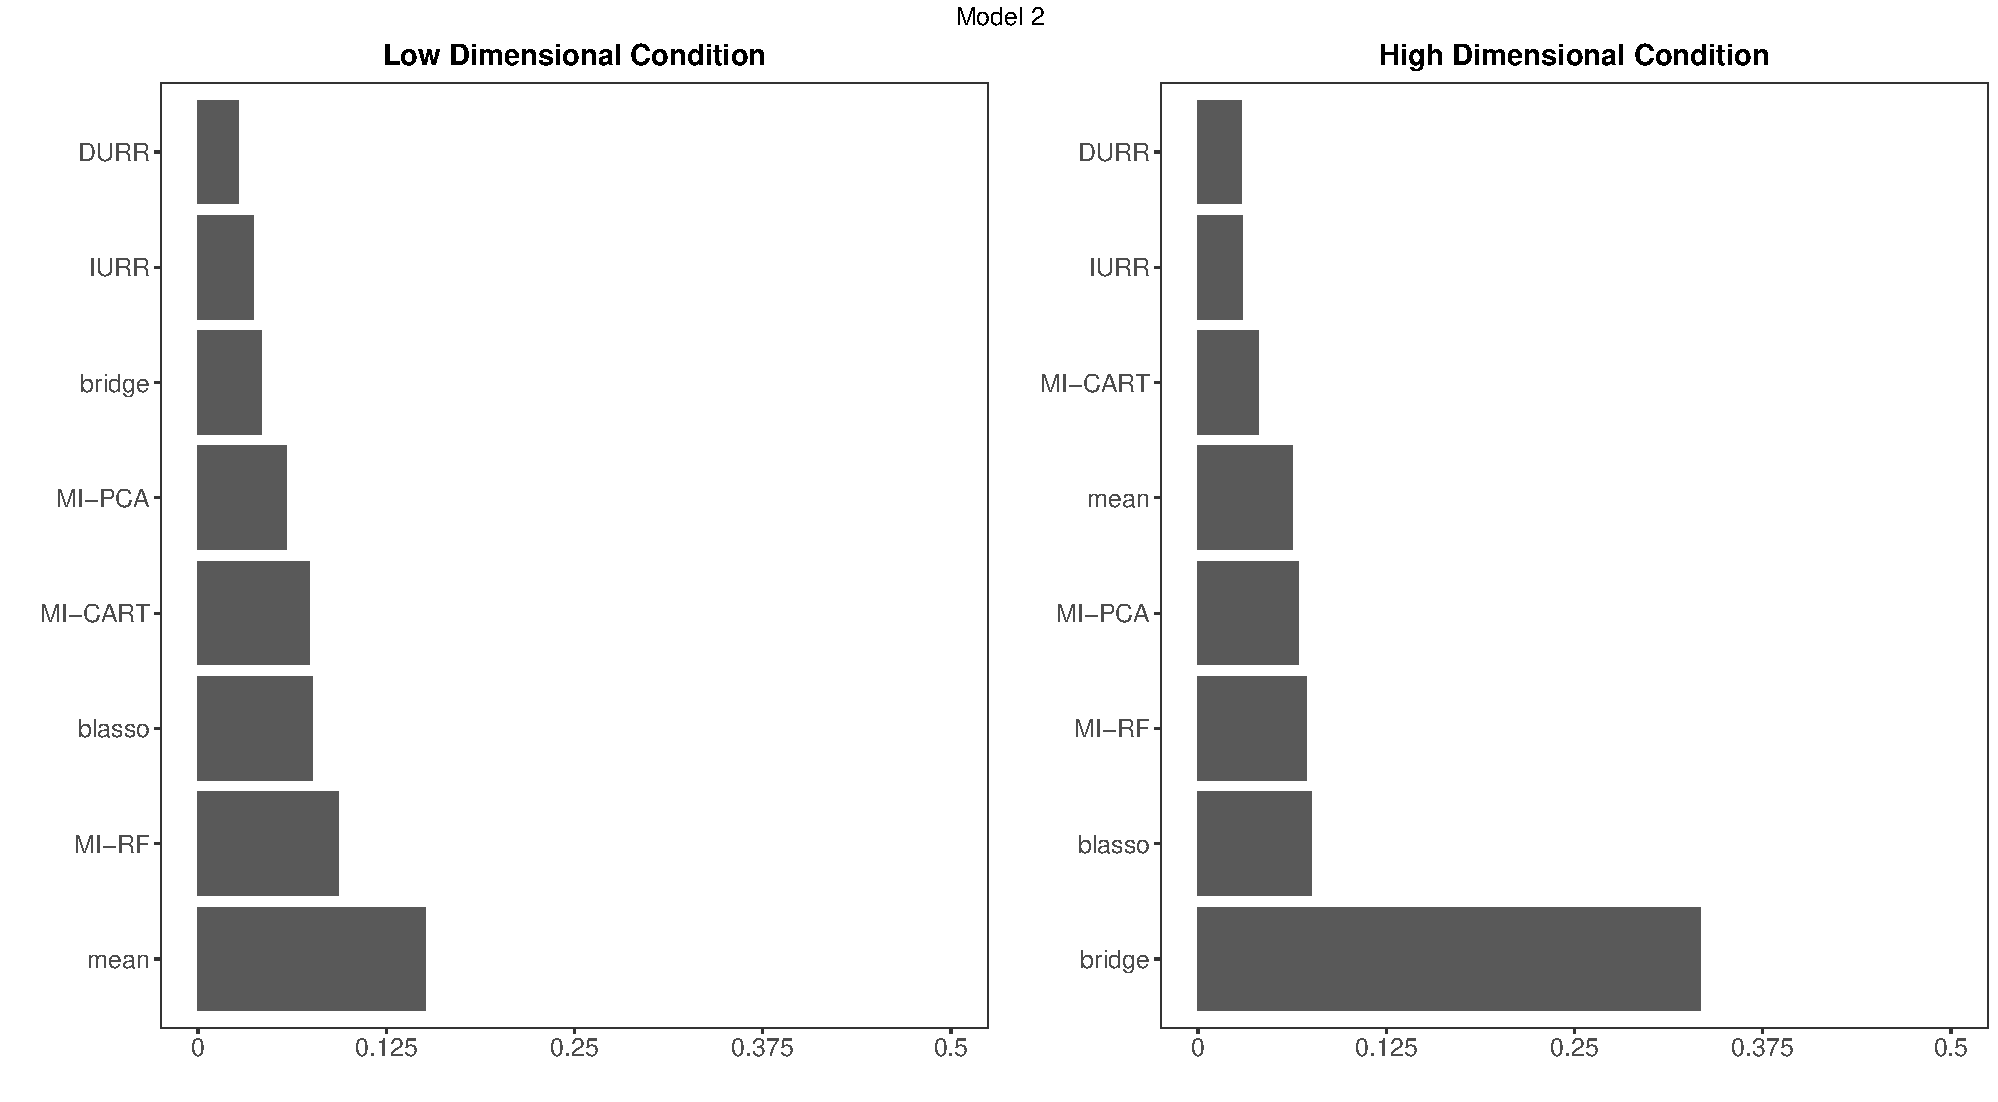
\includegraphics[width=\textwidth]{\pathFIG/exp4_ed_ci.pdf}
	\caption{Euclidean distance between the vector of confidence coverages and the vector of 
		nominal coverage}
	\label{fig:exp4cied}
\end{figure}

\begin{figure}
	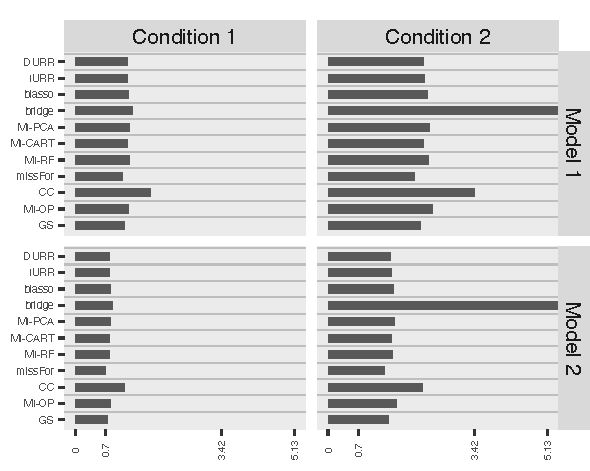
\includegraphics[width=\textwidth]{\pathFIG/exp4_imp_ciw.pdf}
	\caption{Confidence Interval Width for given parameter}
	\label{fig:exp4ciw}
\end{figure}

\FloatBarrier

\subsubsection{Imputation Time}

	Figure \ref{fig:exp4time} shows the average imputation time across the different methods.
	IURR and DURR are the most time consuming methods with imputation times above the hour, 
	in our low dimensional conditions, versus imputation times of a minute or less for MI-PCA and 
	Blasso imputation.
	In the high dimensional condition, the IURR and DURR are not as time-intensive, but still 
	require more then ten times the time of MI-PCA and blasso imputation.

\begin{figure}
	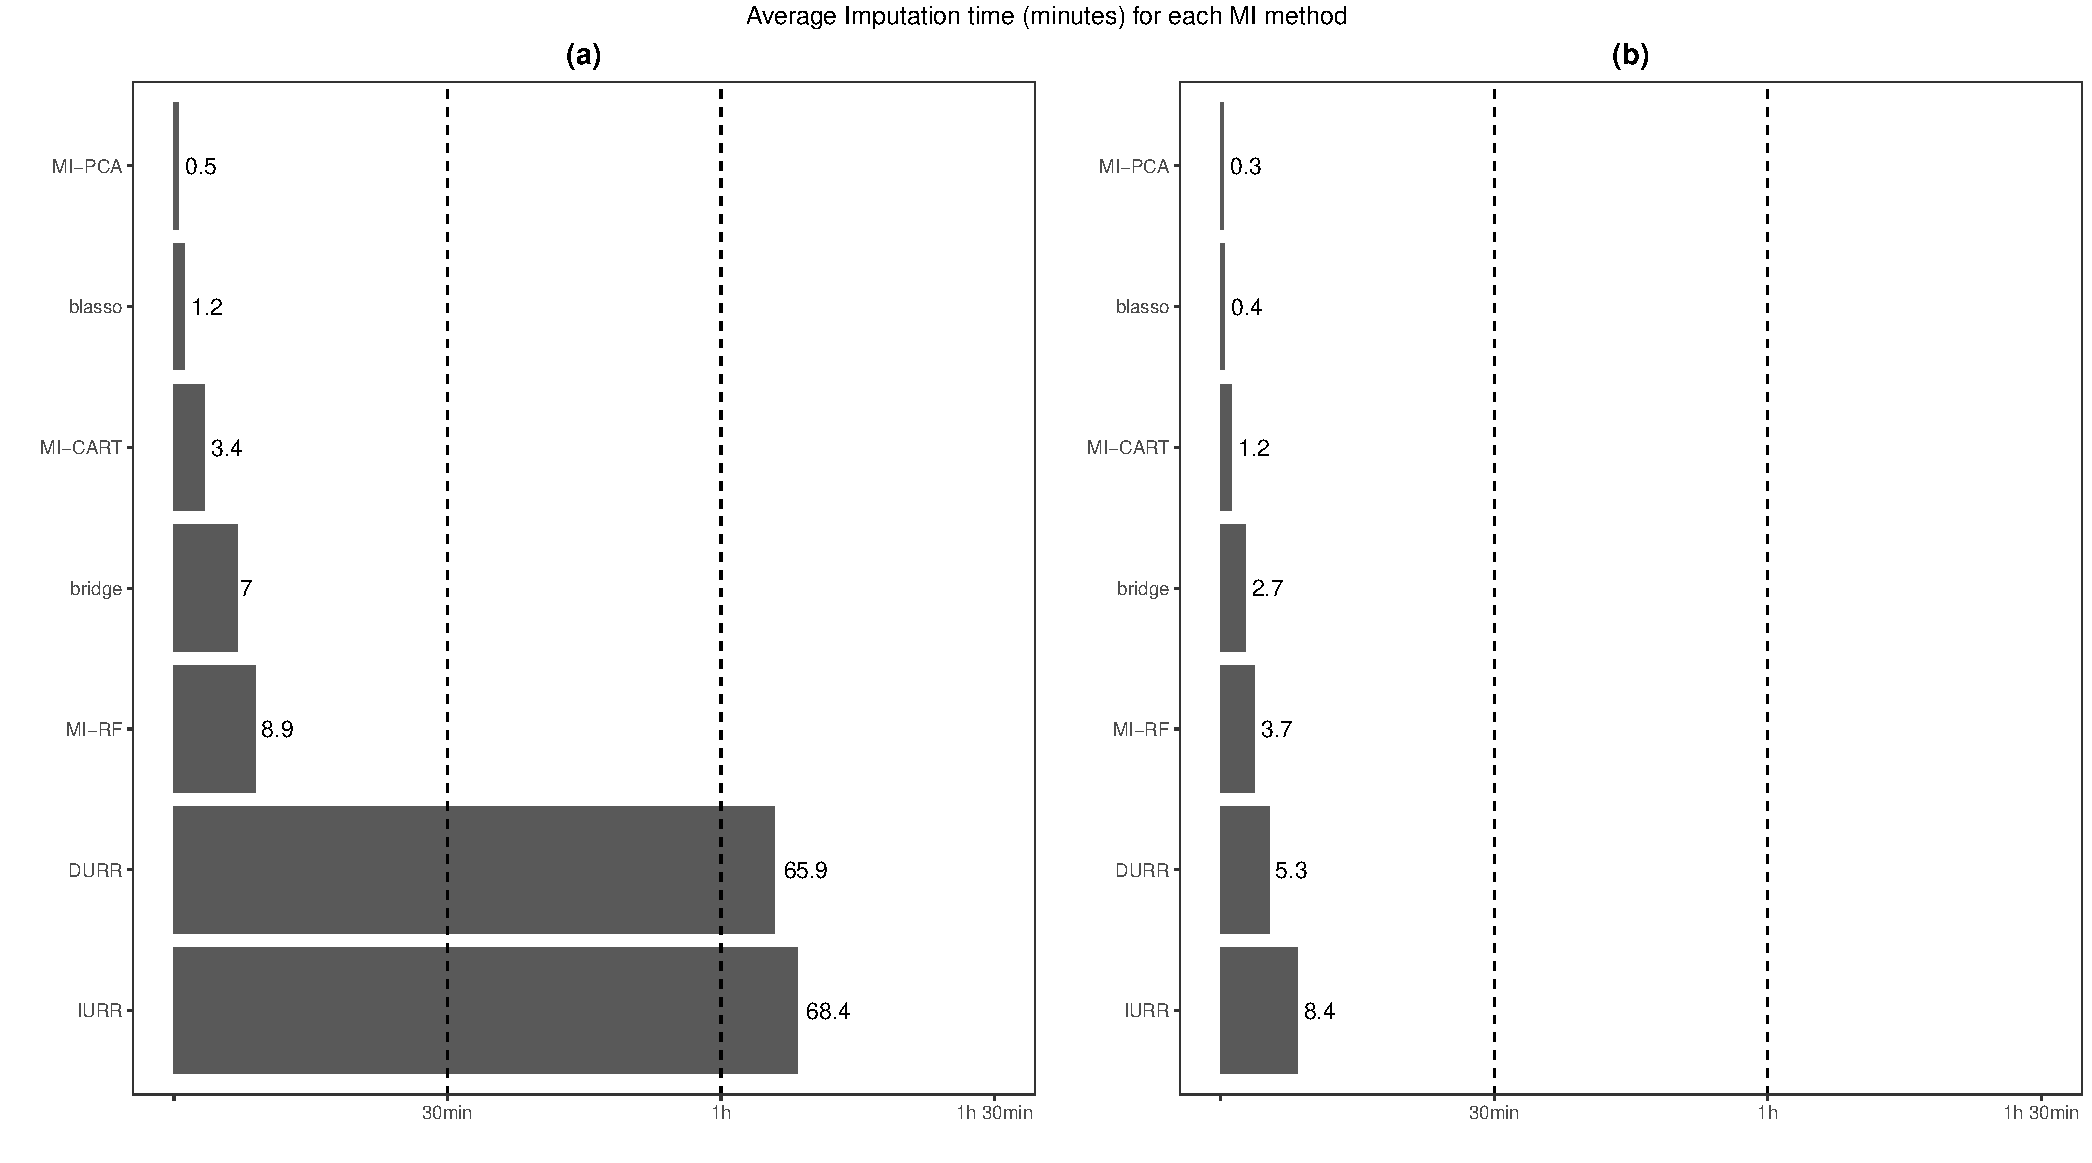
\includegraphics[width=\textwidth]{\pathFIG/exp4_time.pdf}
	\caption{Average imputation time for each method}
	\label{fig:exp4time}
\end{figure}

\FloatBarrier


